\chapter{Estado atual e proximos passos}

\section{O que foi encerrado}

O portao de correcao da scaled dot-product attention esta fechado. As mesmas
entradas, geradas uma unica vez em NumPy, foram executadas em quatro caminhos:
NumPy manual, PyTorch manual, \texttt{torch.nn.functional.scaled\_\allowbreak{}dot\_\allowbreak{}product\_\allowbreak{}attention}
e \texttt{keras.ops.nn.dot\_\allowbreak{}product\_\allowbreak{}attention} com backend TensorFlow. Todas as
nove comparacoes passaram com \texttt{atol=1e-6} e \texttt{rtol=1e-5}; o maior
erro absoluto observado foi $2{,}38418579\times10^{-7}$.

A pipeline de benchmark tambem foi validada em CPU: ela recusa diretorios nao
vazios, captura ambiente antes de persistir resultados, executa lotes
independentes, calcula hashes, grava manifesto e recusa analise quando a
integridade e violada. O diagnostico inicial ainda revelou uma escolha inadequada
de pesos $\mathcal{N}(0,1)$; o contrato foi corrigido para Xavier e a segunda
execucao confirmou a estabilidade de escala esperada.

\section{Proximo passo: coleta na GPU alvo}

\begin{icstatus}[Decisao operacional]{icGreen}
O proximo passo nao e adicionar outro framework nem ampliar a arquitetura. E
clonar este repositorio na maquina com a RTX 4070 Ti Super, validar o ambiente
CUDA e executar a grade principal exatamente como versionada.
\end{icstatus}

\subsection{Preparar o clone}

\begin{Verbatim}[fontsize=\small]
git clone https://github.com/LucasCerqueiraGalvao/scientific-initiation.git
cd scientific-initiation
py -3.11 -m venv .venv
.\.venv\Scripts\python.exe -m pip install --upgrade pip
.\.venv\Scripts\python.exe -m pip install torch==2.11.0+cu128 `
  torchvision==0.26.0+cu128 torchaudio==2.11.0+cu128 `
  --index-url https://download.pytorch.org/whl/cu128
.\.venv\Scripts\python.exe -m pip install `
  -r fases\01_validacao_conceitual\requirements-comparacao.txt
\end{Verbatim}

\subsection{Validar CUDA e dependencias}

\begin{Verbatim}[fontsize=\small]
nvidia-smi
.\.venv\Scripts\python.exe -c "import torch; print(torch.__version__); `
  print(torch.cuda.is_available()); print(torch.cuda.get_device_name(0))"
.\.venv\Scripts\python.exe -m pip check
$env:PYTHONPATH = "fases\01_validacao_conceitual"
.\.venv\Scripts\python.exe -m pytest `
  fases\01_validacao_conceitual\tests -q -W error
\end{Verbatim}

O resultado esperado e \texttt{torch.cuda.is\_\allowbreak{}available() == True}, o nome da
RTX 4070 Ti Super, \texttt{pip check} sem inconsistencias e a suite sem o skip
destinado a ambientes sem CUDA. Qualquer divergencia deve ser registrada antes
da coleta.

\subsection{Revalidar a atencao entre frameworks}

\begin{Verbatim}[fontsize=\small]
.\.venv\Scripts\python.exe -m validacao.comparacao_frameworks `
  --output-dir resultados\comparacao_frameworks_gpu_host `
  --seed 2026 --atol 1e-6 --rtol 1e-5
\end{Verbatim}

Esse comando continua executando TensorFlow em CPU e serve para detectar
mudancas de versao ou ambiente. Nao e benchmark entre frameworks.

\subsection{Executar a grade principal}

O diretorio de saida deve ser novo e vazio. Use uma identificacao com data,
maquina e versao do experimento.

\begin{Verbatim}[fontsize=\small]
$env:PYTHONPATH = "fases\01_validacao_conceitual"
$evidenceDir = "resultados\benchmark_gpu_4070ti_super_YYYY-MM-DD"

.\.venv\Scripts\python.exe -m validacao.benchmark_operacoes `
  --config fases\01_validacao_conceitual\experimentos\benchmark_principal_gpu.json `
  --output-dir $evidenceDir

.\.venv\Scripts\python.exe -m validacao.analise_benchmark_operacoes `
  --evidence-dir $evidenceDir
\end{Verbatim}

\subsection{Critérios de aceite da coleta}

\begin{enumerate}
  \item o runner termina com codigo zero e grava duas execucoes independentes;
  \item o manifesto confirma todos os hashes de CSV e metadados;
  \item nenhuma linha contem NaN ou infinito;
  \item cada candidato e comparado com o baseline da mesma execucao e do mesmo shape;
  \item a analise gera consolidacao, reprodutibilidade e graficos;
  \item o ambiente registra GPU, driver, CUDA, PyTorch, sistema operacional, seed e configuracao;
  \item toda afirmacao de ganho distingue tempo medido, memoria medida, memoria teorica e FLOPs analiticos.
\end{enumerate}

\section{Depois da coleta}

\begin{enumerate}
  \item copiar a evidencia aprovada de \sourcepath{resultados/} para uma pasta versionada em \sourcepath{fases/01_validacao_conceitual/evidencias/benchmarks/};
  \item revisar as diferencas entre as duas execucoes e investigar outliers antes de resumir medias;
  \item responder as perguntas de pesquisa separadamente para projecao densa e self-attention;
  \item confrontar latencia, throughput, memoria e qualidade da saida com o baseline comum;
  \item atualizar este relatorio LaTeX com tabelas, figuras, limitacoes e ameacas a validade;
  \item executar novamente \sourcepath{scripts/build_docs.ps1}, revisar o PDF e publicar o commit de evidencias.
\end{enumerate}

\section{Riscos que permanecem abertos}

\begin{itemize}
  \item pruning nao estruturado pode criar zeros sem acionar um kernel esparso;
  \item quantizacao simulada com dequantizacao pode medir erro numerico sem executar um kernel INT8;
  \item sincronizacao CUDA incorreta distorce latencia; o runner deve continuar usando sincronizacao explicita;
  \item processos em segundo plano, aquecimento termico e clocks variaveis afetam a dispersao;
  \item resultados do ponto CPU nao devem ser usados para prever a ordem relativa na GPU;
  \item uma conclusao global exige separar os resultados por operacao, shape e metrica.
\end{itemize}

\begin{figure}[H]
  \centering
  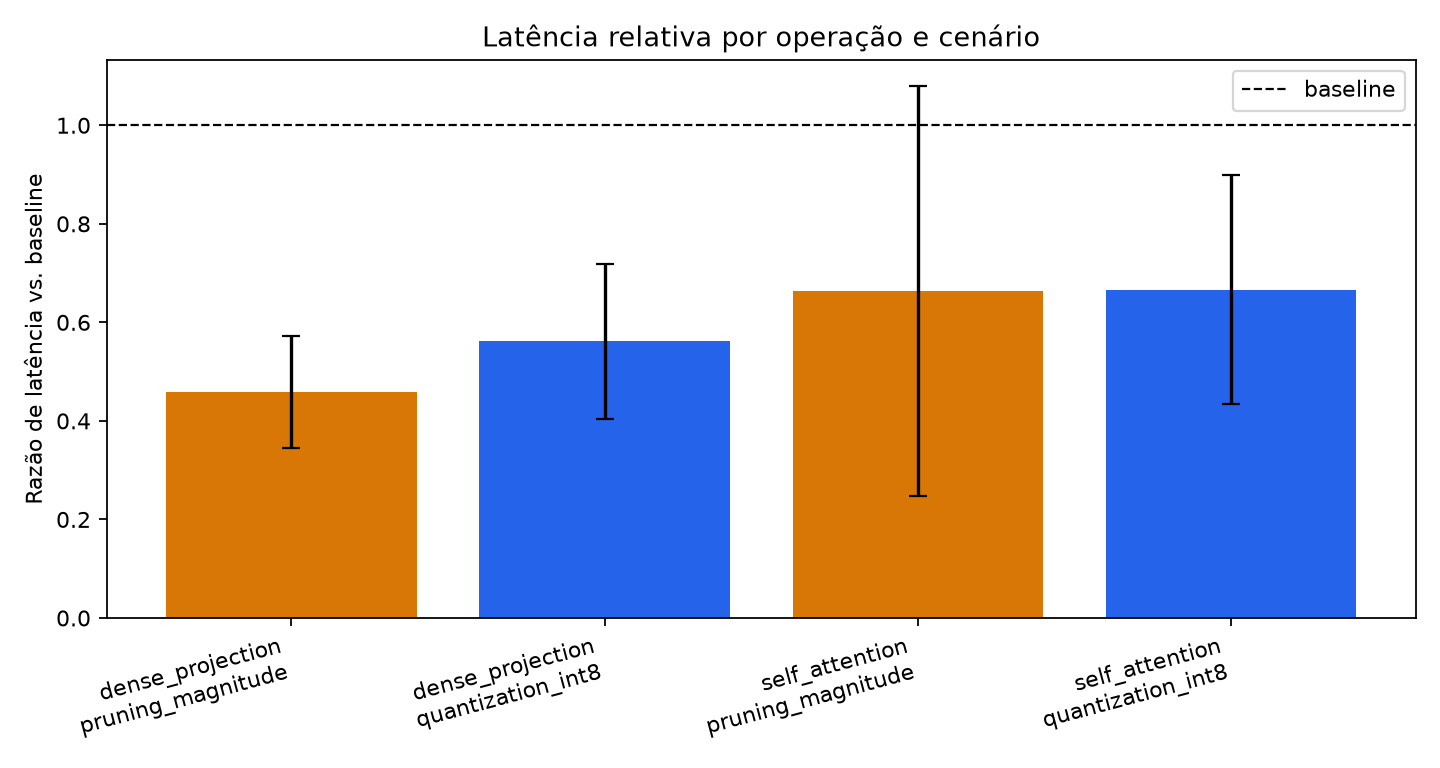
\includegraphics[width=0.76\linewidth]{fases/01_validacao_conceitual/evidencias/benchmarks/diagnostico_cpu_l64_d128_v2_2026-08-25/analise/latencia_relativa.png}
  \caption{Diagnostico CPU v2. A figura valida a pipeline de analise, nao o desempenho do hardware alvo.}
\end{figure}

\begin{figure}[H]
  \centering
  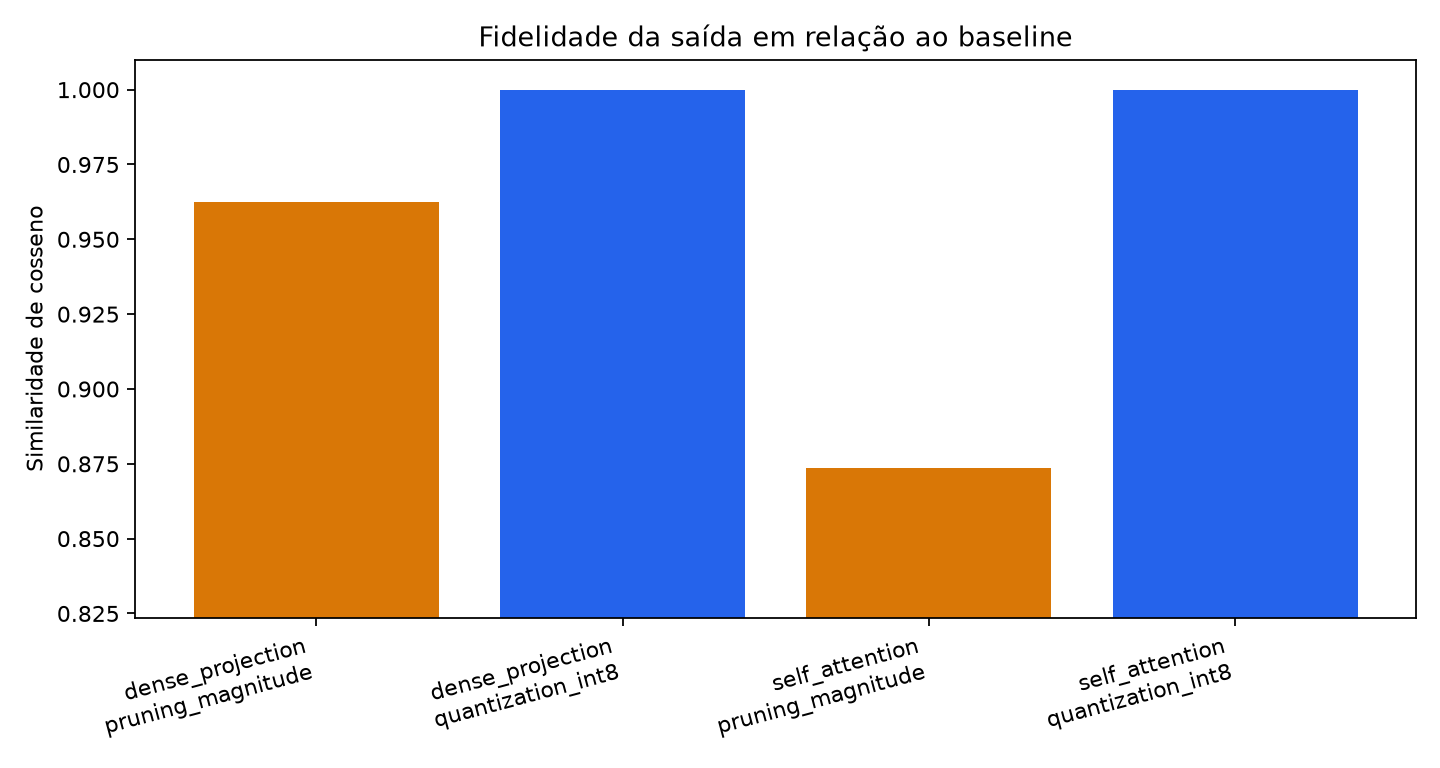
\includegraphics[width=0.76\linewidth]{fases/01_validacao_conceitual/evidencias/benchmarks/diagnostico_cpu_l64_d128_v2_2026-08-25/analise/qualidade_saida.png}
  \caption{Qualidade numerica das saidas no diagnostico CPU v2.}
\end{figure}
